\section{Activated Recurrence}
The wave alone rejects every multiple of its modulus, including the modulus
itself. That would remove each prime when its own filter is installed. We
therefore activate a filter only after its own integer.

\begin{itemize}
\item A uniform update at every integer filter.
\item Nonnegative height increments and protection of earlier inputs.
\end{itemize}

For $m\ge2$ and $t\ge2$, put
\begin{equation*}
\begin{aligned}
a_m(t)&=\min(1,\max(0,t-m)),\\
F_1(t)&=t+i\sin^2(\pi t),\\
F_M(t)&=F_{M-1}(t)+i a_M(t)W_M(t)\quad(M\ge2).
\end{aligned}
\end{equation*}

The activation is zero through $m$, rises linearly to one at $m+1$, and
stays one afterwards. Every integer is a contact of $F_1$. Each update adds
imaginary height at later multiples of its index, leaving all other integer
heights unchanged. The index runs through every integer; no primality test
is needed to choose the next filter.

Write $F_M(t)=t+i h_M(t)$. Each stage is continuous and its real coordinate
is still $t$. Successive substitution in the recurrence gives one finite sum:
\begin{equation*}
\begin{aligned}
F_M(t)-F_1(t)
&=\sum_{m=2}^{M}\bigl(F_m(t)-F_{m-1}(t)\bigr)
&&[\text{Telescoping}]\\
&=i\sum_{m=2}^{M}a_m(t)W_m(t).
&&[\text{By Definition}]
\end{aligned}
\end{equation*}

Consequently,
\begin{equation*}
\begin{aligned}
h_M(t)&=\sin^2(\pi t)+\sum_{m=2}^{M}a_m(t)W_m(t),\\
h_M(t)-h_{M-1}(t)&=a_M(t)W_M(t)\ge0\quad(M\ge2).
\quad[\text{Nonnegativity}]
\end{aligned}
\end{equation*}

The finite-sum formula includes $M=1$, with an empty sum. Nonnegative increments
mean that a rejected value cannot become a contact again. At a fixed input,
filters only raise the curve; they cannot cancel earlier height.

The protection also applies to a whole real interval. When $2\le t\le M$,
$a_M(t)=0$, hence
\begin{equation*}
\begin{aligned}
F_M(t)&=F_{M-1}(t)\quad(M\ge2,\ 2\le t\le M).
\quad\blacksquare\ \text{[Q.E.D.]}
\end{aligned}
\end{equation*}

This protects the earlier curve from the incoming filter. It does not say
that every earlier integer has zero height: previous filters may already
have rejected a composite there. Between later integers a wave may alter the
curve even where its samples at neighboring integers vanish.

For example, filter $4$ contributes zero at $4,5,6,7$, contributes one at
$8$, and contributes zero at $9,10,11$. The extra height at $8$ records
another divisor, although filter $2$ has already rejected that integer.

Figure~\ref{fig:activated-filter-4} isolates this single filter. The dashed
wave reaches one at $4$, but activation leaves the contribution zero there;
later multiples $8$ and $12$ receive one unit. The plot shows one filter
contribution, not the total height $h$.

\begin{figure}[htbp]
\centering
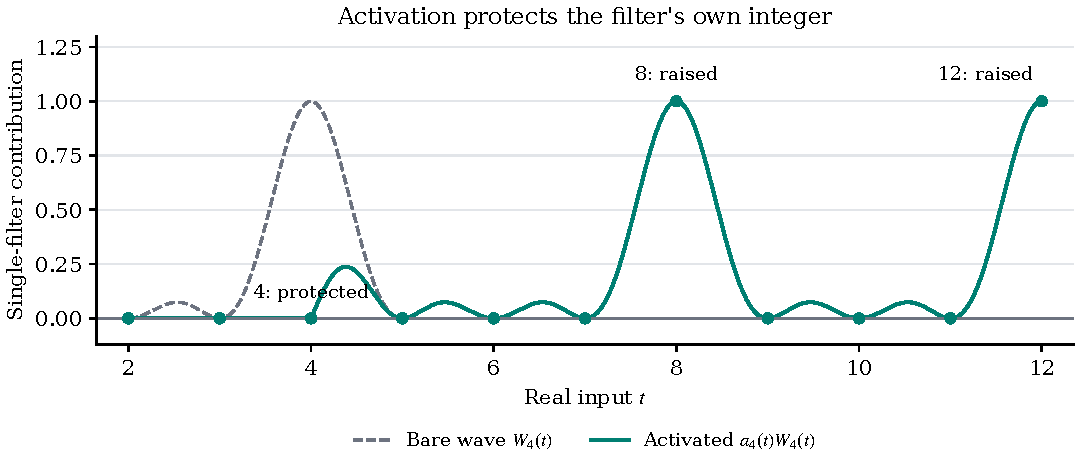
\includegraphics[width=\textwidth]{figures/activated-filter-4.pdf}
\caption{Bare and activated filter $4$ on $[2,12]$. The dashed curve is
$W_4(t)$ and the solid curve is $a_4(t)W_4(t)$; the markers are exact integer
samples. This is a single-filter contribution, not the total height. The
figure is generated from the definitions above by the static plotting script
in the project repository.}
\label{fig:activated-filter-4}
\end{figure}
